\documentclass[a4paper, 12pt, oneside]{report}

\usepackage[utf8]{inputenc}
\usepackage{lmodern}
\usepackage{layout}
\usepackage{emptypage}
\usepackage{fancyhdr}
\usepackage{fancyref}
\usepackage{fancyvrb}
\usepackage{subcaption} % subfiguras
\usepackage{caption}
\usepackage{mathtools}
\usepackage{hyperref}
\usepackage[a4paper,top=3cm, bottom=3cm, inner=2.5cm, outer=2.5cm]{geometry}
\usepackage{listings}
\usepackage[english]{babel}
\usepackage{url}
\usepackage{color}
\usepackage{natbib}
\usepackage{amsmath}
\usepackage{algorithm}
\usepackage{amsmath}
\usepackage[noend]{algpseudocode}

\definecolor{codegreen}{rgb}{0,0.6,0}
\definecolor{codegray}{rgb}{0.5,0.5,0.5}
\definecolor{codepurple}{rgb}{0.58,0,0.82}
\definecolor{backcolour}{rgb}{0.95,0.95,0.92}

\lstset{frame=single,
	language=Python,
	aboveskip=3mm,
	belowskip=3mm,
	showstringspaces=false,
	columns=flexible,
	basicstyle={\small\ttfamily},
	numbers=none,
	backgroundcolor=\color{backcolour},   
	commentstyle=\color{codegreen},
	keywordstyle=\color{blue},
	numberstyle=\color{codepurple},
	stringstyle=\color{magenta},
	breaklines=true,
	breakatwhitespace=true,
	tabsize=3
}

%\usepackage{titlesec}
\makeatletter
\renewcommand{\@makeschapterhead}[1]{
  \vspace*{0\p@}%
  {\parindent \z@ \raggedright
    \normalfont
    \interlinepenalty\@M
    \Huge \bfseries  #1\par \nobreak
    \vskip 15\p@
  }}
\makeatother

\renewcommand{\baselinestretch}{1.4}
\setlength{\headheight}{16pt} 

\pretolerance=1000

\chead[]{}
\rhead[]{}
\renewcommand{\headrulewidth}{0.5pt}

\pagestyle{empty}

\title{Vehicle Detection using Deep Learning}
\author{David Pascual Hernández}

\begin{document}
%%%%%%%%%%%%%%% Cover %%%%%%%%%%%%%%%%%%%%
\begin{titlepage}
	
	\begin{center}
		
		\begin{figure}[htb]
			\begin{center}
				
\includegraphics[width=0.6\linewidth]{figures/logo}
			\end{center}
		\end{figure}
		
		\vspace{10mm}
		
		\begin{Large}
			\textbf{ESCUELA TECNICA SUPERIOR DE INGENIERÍA DE TELECOMUNICACIÓN}
			\vspace{10mm}
		\end{Large}
		
		\begin{Large}
			Grado en Ingeniería en\\ \vspace{2mm} Sistemas Audiovisuales y Multimedia
		\end{Large}
		
		\vspace{10mm}
		
		\begin{large}
			\textbf{Trabajo Fin de Grado}
		\end{large}
		\vspace{25mm}
		
		\begin{huge}
			Study of Convolutional Neural Networks with Keras
		\end{huge}
		
		\vspace{25mm}
		
		\begin{large}
			\textbf{Autor}: David Pascual Hernández
			
			\textbf{Tutor}: José María Cañas Plaza
			
			\textbf{Co-tutor}: Inmaculada Mora Jiménez 
			
			\vspace{10mm}
			
			Curso académico 2016/2017
		\end{large}
		
		\vspace{10mm}
		
	\end{center}
	
\end{titlepage}

\pagebreak
\thispagestyle{empty}
\vspace*{12cm}

\begin{flushright}
	
	
\includegraphics[height=1.0cm]{figures/CC-BY-SA.png}
	
	\vspace*{0.5cm}
	
	\copyright 2017 David Pascual Hernández
	
	\vspace*{0.3cm}
	
	Esta obra está distribuida bajo la licencia de 
	
	``Reconocimiento-CompartirIgual 4.0 Internacional (CC BY-SA 4.0)''
	
	de Creative Commons.
	
	\vspace{0.2cm}
	
	Para ver una copia de esta licencia, visite
	
	http://creativecommons.org/licenses/by-sa/4.0/ o envíe
	
	una carta a Creative Commons, 171 Second Street, Suite 300,
	
	San Francisco, California 94105, USA.
	
\end{flushright}

\pagenumbering{Roman}

%%%%%%%%%%%%%%% Acknowledgements %%%%%%%%%%%%
\include{0-Acknowledgements}

%%%%%%%%%%%%%%% Overview %%%%%%%%%%%%%%%%%%%%
\include{0-Overview}

%%%%%%%%%%%%%%% Índices %%%%%%%%%%%%%%%%%%%%
\tableofcontents
\listoffigures % Í­ndice de figura
\cleardoublepage

%%%%%%%%%%%%%%% Chapters %%%%%%%%%%%%%%%%%%
\pagestyle{fancy}
\pagenumbering{arabic}
\setlength{\parindent}{6mm}

\lhead[]{CHAPTER \thechapter. ABSTRACT}
\include{1-Abstract}
\lhead[]{CHAPTER \thechapter. GOALS}
\include{2-Goals}
\lhead[]{CHAPTER \thechapter. FRAMEWORK}
\chapter{Framework}\label{ch:framework}
This chapter serves as a way to introduce the tools that have been employed during the development of this project. All of them are \textbf{open-source}. The transparency provided by the open-source platforms is a major advantage, because the software can be joined together and adapted to our specific applications, which are mainly written in \textbf{Python} \footnote{\url{https://www.python.org/}}.

\section{JdeRobot}\label{sec:jderobot}
\textbf{JdeRobot} \cite{jderobot} is an open source middleware for robotics and computer vision. It has been designed to simplify the software development within these fields. It's mostly written in C\nolinebreak[4]\hspace{-.05em}\raisebox{.4ex}{\tiny\bf ++} language and it's structured like a collection of components (tools and drivers) that communicate to each other through \textbf{ICE interfaces} \footnote{\url{https://zeroc.com/products/ice}}. It is also compatible with \textbf{ROS} \footnote{\url{http://www.ros.org/}}, which allows the interoperation of ROS nodes and JdeRobot components. This flexibility makes it very useful for our application.
Its \textbf{\textit{cameraserver} driver} is going to be employed to capture images from different video sources.

\subsection{\textit{cameraserver}}\label{subsec:cameraserver}
According to JdeRobot documentation \cite{jderobot}, this driver can serve both real cameras and video files. It communicates with other components thanks to the \textbf{\textit{Camera} interface}.

In order to use \textbf{\textit{cameraserver}}, its configuration file has to be properly set. These are the parameters that must be specified:
\begin{itemize}
    \item The \textbf{network address} where the server is going to be listening.
    
    \item Parameters related with the \textbf{video stream}: URI, frame rate, image size and format.
\end{itemize}

\section{MNIST}\label{sec:MNIST}
\textbf{MNIST (Modified National Institute of Standards and Technology database)} \cite{lecun-mnisthandwrittendigit-2010} is a database of \textbf{handwritten digits} formed by a training set, which contains 60000 samples, and a test set, containing 10000 samples. It's a \textit{remixed} and reduced version of the original \textbf{NIST datasets} \footnote{\url{https://www.nist.gov/srd/nist-special-database-19}}. MNIST is a well-known \textbf{benchmark} for all kinds of machine learning algorithms.

As may be seen in figure \ref{fig:mnist}, each sample of the MNIST database is a 28x28 pixels \textbf{grayscale image} that contains a \textbf{size-normalized} and \textbf{centered} digit. While it may be useful for testing machine learning algorithms, it's not enough to train a model that aims to solve a \textbf{real-world task}, because the images are almost noiseless and share similar orientation, position, size and intensity levels. The dataset must be \textbf{augmented} to face this problem \ref{subsec:datasets}.
\begin{figure}
	\centering
	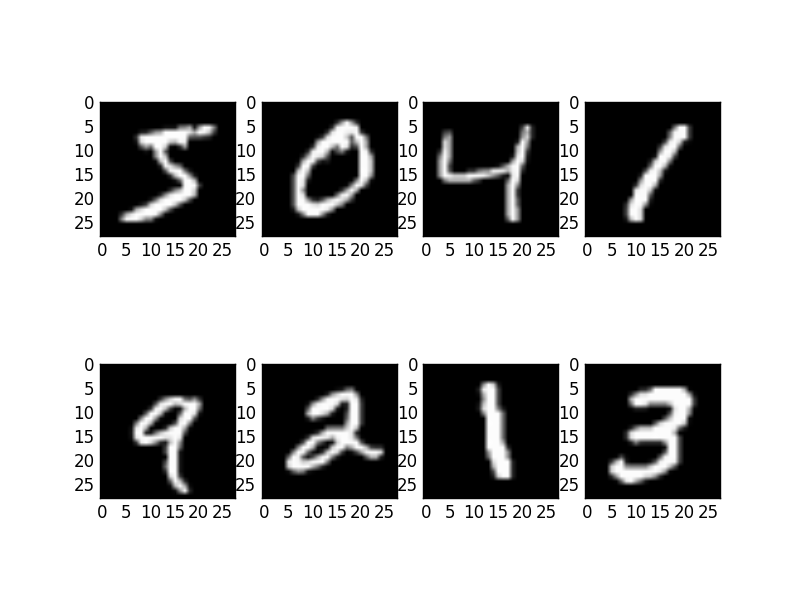
\includegraphics[width=12cm, keepaspectratio]{figures/mnist.png}
	\caption{Samples extracted from the MNIST database}
	\label{fig:mnist}
\end{figure}

\section{Keras}\label{sec:keras}
As stated by \textbf{Keras} documentation \cite{chollet2015keras}: "Keras is a high-level \textbf{neural network library}, written in Python and capable of running on top of either TensorFlow or Theano". TensorFlow and Theano are open-source libraries for numerical computation optimized for GPU and CPU that Keras treats as its \textit{backends}. In this project, Keras is running on top of \textbf{Theano} \footnote{\url{http://deeplearning.net/software/theano/index.html}} optimized for CPU, but it's quite easy to switch from one backend to another.

In the following sections, the main elements that make up a neural network built with Keras are going to be analyzed, starting with the \textbf{\textit{model} object}, its core component.

\subsection{Models}\label{subsec:models}
Every neural network in Keras is defined as a \textbf{\textit{model}}. For those models which can be built as a stack of \textit{layers} \ref{subsec:layers}, Keras provides the \textbf{\textit{.Sequential()} object}. An example of a sequential model built with Keras can be seen in figure \ref{fig:model}. It is also possible to build more complex models with multiple outputs and shared layers using the \textbf{Keras functional API}.
\begin{figure}
	\centering
	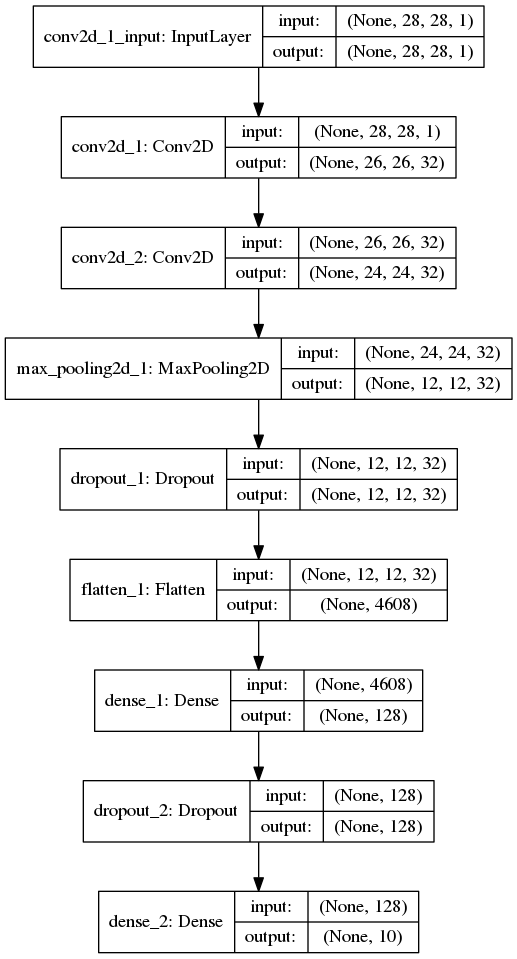
\includegraphics[width=0.75\linewidth, keepaspectratio]{figures/model.png}
	\caption{Diagram of a Keras sequential model}
	\label{fig:model}
\end{figure}

Sequential models have several methods, and the following ones are essential for the learning process:
\begin{description}
	\item[\textit{.compile()}] It configures the learning process. It's main arguments are:
	\begin{itemize}
		\item \textbf{\textit{loss}}: name of the \textbf{cost function} employed to check the difference between the predicted label and the real one. In this project, the \textbf{categorical cross-entropy}, also known as log loss, has been used. It returns the cross-entropy between an approximating distribution $q$ and a true distribution $p$ \cite{2016arXiv160502688short} and it's defined as:
		\begin{equation}\label{eq:categorical_crossentropy}
		H(p,q)=-\Sigma_{x}p(x)\log(q(x))
		\end{equation}		
		Other loss functions such as mean squared error (MSE), mean absolute error and hinge are also provided by Keras.
		
		\item \textbf{\textit{optimizer}}: name of the optimizer that will update the weights values during training in order to minimize the loss function. The chosen algorithm for this task is \textbf{ADADELTA} \cite{DBLP:journals/corr/abs-1212-5701}. This optimizer is an extension of the \textbf{gradient descent} optimization method that has the particularity of adapting the learning rate during training with no need of manual tuning. It follows the next algorithm \cite{DBLP:journals/corr/abs-1212-5701}:
		
		\begin{minipage}{\linewidth}
		\begin{algorithm}[H]
			\caption{Computing ADADELTA update at time $t$}\label{adadelta}
		  	\begin{algorithmic}[1]
		  		\Require{Decay rate $\rho$, Constant $\epsilon$}
		  		\Require{Initial parameter $x_1$}
		  		\State Initialize accumulation variables $E[g^2]_0=0, E[\Delta x^2]_0 = 0$
		  		\For{$t=1:T$} \Comment{Loop over \# of updates}
		  		\State Compute gradient: $g_t$
		  		\State Accumulate gradient: $E[g^2]_t=\rho E[g^2]_{t-1}+(1-\rho)g_t^2$
		  		\State Compute update: $\Delta x_t=-\frac{\mathrm{RMS}[\Delta x]_{t-1}}{\mathrm{RMS}[g]_t}g_t$
		  		\State Accumulate updates: $E[\Delta x^2]_t=\rho E[\Delta x^2]_{t-1}+(1-\rho)\Delta x_t^2$
		  		\State Apply update: $x_{t+1}=x_t+\Delta x_t$
				\EndFor
		  		\State \textbf{end for}
		  	\end{algorithmic}
		\end{algorithm}
		\end{minipage}\\
				
		Other optimization methods such as Adagrad, Adamax and Adam are also available.
		
		\item \textbf{\textit{metrics}}: name of the parameters that must be evaluated during training and testing. The only metric that is going to be calculated with Keras through this project, besides the result of the loss function which is automatically computed, is \textbf{accuracy}. It is defined as the proportion of examples for which the model produces the correct output \cite{Goodfellow-et-al-2016}.			
		Other metrics are calculated with \textbf{Scikit-learn} \ref{sec:sklearn} library, in order to obtain a evaluation of the model that is independent from Keras.
	\end{itemize}
\end{description}

\begin{description}
	\item[\textit{.fit()}] It trains the model. The following arguments are required:
	\begin{itemize}
		\item \textbf{\textit{x}, \textit{y}}: training samples and labels. They must be defined as \textbf{Numpy arrays}\footnote{\url{http://www.numpy.org/}}.
		
		\item \textbf{\textit{batch\_size}}: number of samples that are evaluated before updating the weights. It defaults to 32.
		
		\item \textbf{\textit{epochs}}: number of iterations over the whole dataset that are going to be executed. It defaults to 10.
		
		\item \textbf{\textit{callbacks}}: list of callbacks \ref{subsec:callbacks} that are going to be applied during training. It defaults to \textit{None}.
		
		\item \textbf{\textit{validation\_split} or \textit{validation\_data}}: On one hand, \textit{validation\_split} defines the fraction of the training data that has to be used as held-out validation data. On the other hand, \textit{validation\_data} is a tuple containing the samples and labels of a validation dataset provided by the user. They are mutually exclusive.
		
		\item \textbf{\textit{shuffle}}: a boolean that determines whether to shuffle training data or not. 
	\end{itemize}
\end{description}

\begin{description}
	\item[\textit{.evaluate()}] It takes a set of samples and labels and evaluates the \textbf{model performance}, returning a list of the metrics previously defined.
\end{description}

\begin{description}
	\item[\textit{.predict()}] It takes a sample and returns the label predicted by the model.
\end{description}

\begin{description}
	\item[\textit{.save()}] It stores the model into a \textbf{HDF5 file} \ref{sec:hdf}, which will contain the weights, architecture and training configuration of the model.
\end{description}

\begin{description}
	\item[\textit{.load\_model()}] It loads a model from a \textbf{HDF5 file}.
\end{description}

\subsection{Layers}\label{subsec:layers}
As it has been said before, the models are usually built as a \textbf{stack of layers}. These layers are added to the model using the \textbf{\textit{.add()} method}, inside of which the kind of layer is declared and its particular parameters are set. Several kinds of layers are available, but only the ones that have been used in this project are going to be described.
\begin{description}
	\item[Convolutional layer] This particular layer is the one that turns the neural network into a \textbf{convolutional neural network (CNN)}. It is formed by a fixed number of \textbf{filters/kernels} with a fixed size. These filters are convolved along the input image, generating each one a \textbf{feature or activation map} which will tell us to what extent the feature learned by that particular filter is present in the input image \cite{cs231n}. It's important to note that the \textit{depth} of the filter will be equal to the number of channels of the input, which implies that each filter will generate just one activation map, instead of generating one for each channel. 
	
	Keras provides different kinds of convolutional layers depending on the input dimensions: \textit{Conv1D}, \textit{Conv2D} and \textit{Conv3D}. These are the main arguments required by Keras to define a convolutional layer:
	\begin{itemize}
		\item \textbf{\textit{filters}}: number of filters.
		
		\item \textbf{\textit{kernel\_size}}: width and height of the filters.
		
		\item \textbf{\textit{strides}}: how many pixels the filter must be shifted before applying the next convolution. Output size depends on this parameter. It defaults to 1.
		
		\item \textbf{\textit{padding}}: it can be \textit{valid} or \textit{same}. If \textit{valid} mode is set, no padding is applied, resulting in a reduced output. However, if \textit{same} mode is set, the input will be padded with zeros in order to produce an output that preserves the input size. It defaults to \textit{valid}.
	\end{itemize}

	Figure \ref{fig:convlayer} shows how the convolutional layers work. 
	
	\begin{figure}
		\centering
		\begin{subfigure}{0.65\textwidth}
			\centering
			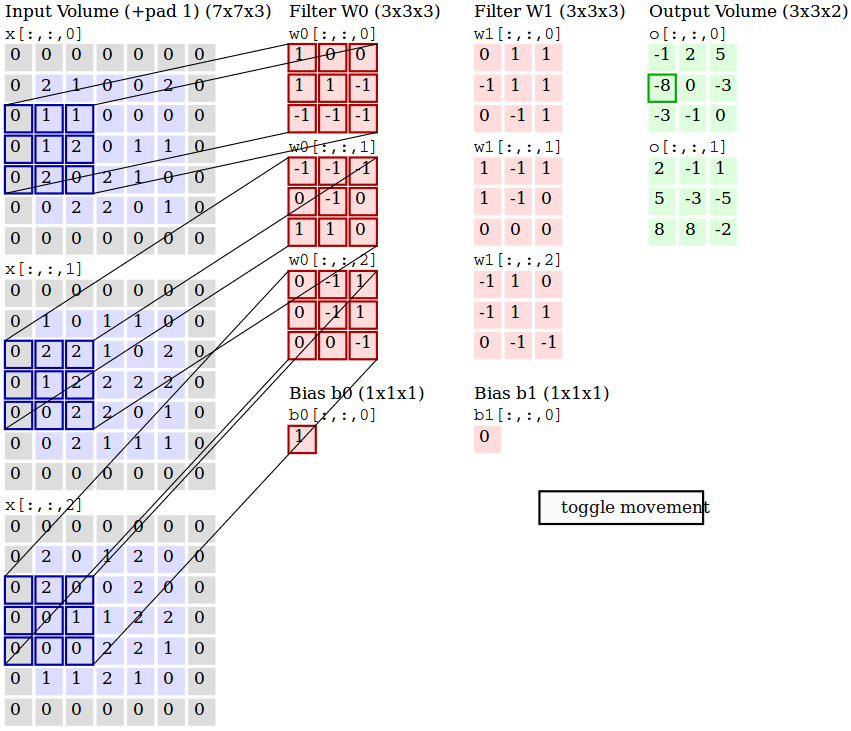
\includegraphics[width=1\linewidth]{figures/convlayer_anime1big.png}
			\caption{}\label{fig:conv_a}
		\end{subfigure}
		\begin{subfigure}{0.65\textwidth}
			\centering
			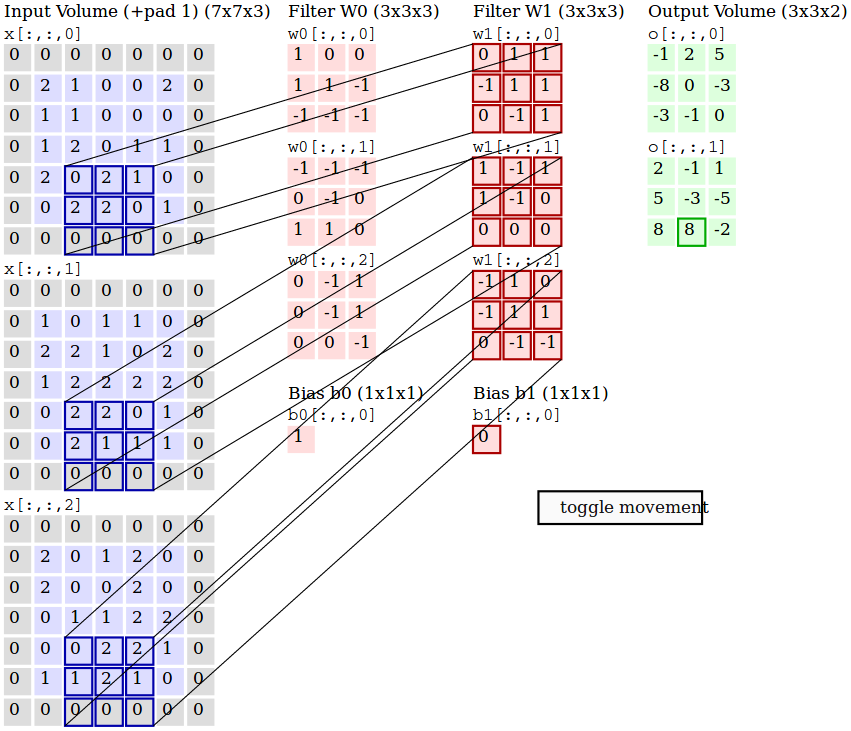
\includegraphics[width=1\linewidth]{figures/convlayer_anime2big.png}
			\caption{}\label{fig:conv_b}
		\end{subfigure}
		\caption[Convolutional layer]{In the figure \ref{fig:conv_a}, the filter $w_0$ (3x3x3) is convolved with the input image (5x5x3). As padding is set to 1 pixel around the input and the stride is equal to 2 pixels, the operation will return a 3x3 activation map. The same procedure is followed in the figure \ref{fig:conv_b} with the filter $w_1$. It generates another 3x3 activation map, ending up with a 3x3x2 output (depth = number of filters = 2). These images have been extracted from \cite{cs231n}}
		\label{fig:convlayer}
	\end{figure}
	
\end{description}

\begin{description}
	\item[{Pooling layer}] It shifts a window of a certain size along the input image applying an operation (mean or maximum) that will return a \textbf{\textit{downsampled} version} of it, reducing the computational cost and avoiding over-fitting \cite{Scherer2010Evaluation}. Figure \ref{fig:pooling} shows how the pooling operation is applied.

	\begin{figure}
		\centering
		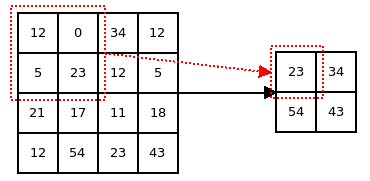
\includegraphics[width=10cm, keepaspectratio]{figures/pooling.png}
		\caption{Example of a max. pooling operation}
		\label{fig:pooling}
	\end{figure}
	
	Depending on the dimensions of the input and the operation applied, Keras provides several pooling layers: \textit{MaxPooling1D}, \textit{MaxPooling2D}, \textit{MaxPooling3D}, \textit{AveragePooling1D}... The main arguments required by Keras to define these layers are:
	\begin{itemize}
		\item \textbf{\textit{pool\_size}}: size of the window that is shifted along the input. It can also be interpreted as the factor by which the input is going to be downsampled.
		\item \textbf{\textit{strides}}: how many pixels the window must be shifted before applying the next operation.
	\end{itemize}
\end{description}

\begin{description}
	\item[Dense layer] Fully-connected layers in Keras are defined as \textit{Dense layers}. In a \textbf{fully-connected layer}, every neuron is connected to every activation (output) of the previous one \cite{cs231n}. The main argument of this layer is:
	\begin{itemize}
		\item \textbf{\textit{units}}: number of neurons.
	\end{itemize} 
\end{description}

\begin{description}
	\item[Activation layers] In Keras models, activations can be declared as a layer itself, or as an argument within the \textit{.add()} method of the previous layer. Keras provides several \textbf{activation functions}, such as sigmoid, linear, ReLU and softmax. The only argument that must be provided to activation layers is the name of the desired activation function. These are the ones that have been used during the development of this project:
	\begin{itemize}
		\item \textbf{ReLU (Rectified Linear Unit)}: This activation function introduces \textbf{non-linearity} right after each convolutional layer, allowing the CNN to learn more complex features. It's defined as:
		\begin{equation}\label{eq:ReLU}
		g(z)=\max(0,z)
		\end{equation}
		
		\item \textbf{Softmax} This activation function is very useful when is placed after the \textbf{output layer} of classification tasks. It takes a vector of real values $z$ and returns a new vector of real values in the range [0,1]. The $N$ elements of the output vector can be considered \textbf{probabilities} because the softmax function ensures that they sum up to 1. It is defined as follows:
		\begin{equation}\label{eq:SoftMax}
		\mathrm{softmax}(z)_i=\frac{\exp(z_i)}{\Sigma_{j}{\exp(z_j)}} \quad \mathrm{for} \ j=1, ...,N
		\end{equation}
	\end{itemize}
	These equations have been extracted from \cite{Goodfellow-et-al-2016}. Figure \ref{fig:activations} shows these activation functions plotted in the interval [-1,1].

	\begin{figure}
		\centering
		\begin{subfigure}{0.5\textwidth}
			\centering
			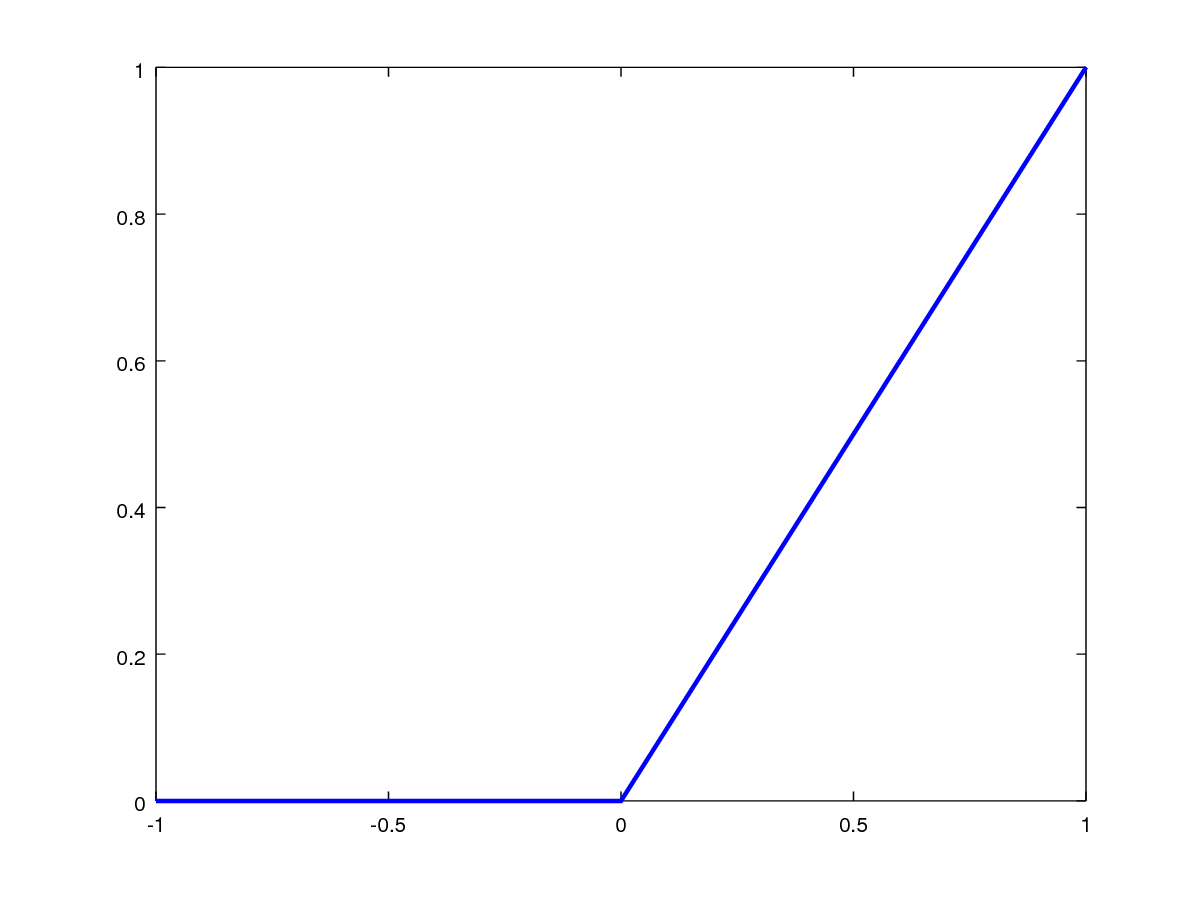
\includegraphics[width=1\linewidth]{figures/relu.png}
			\caption{ReLU activation function}\label{fig:relu}
		\end{subfigure}%
		\begin{subfigure}{0.5\textwidth}
			\centering
			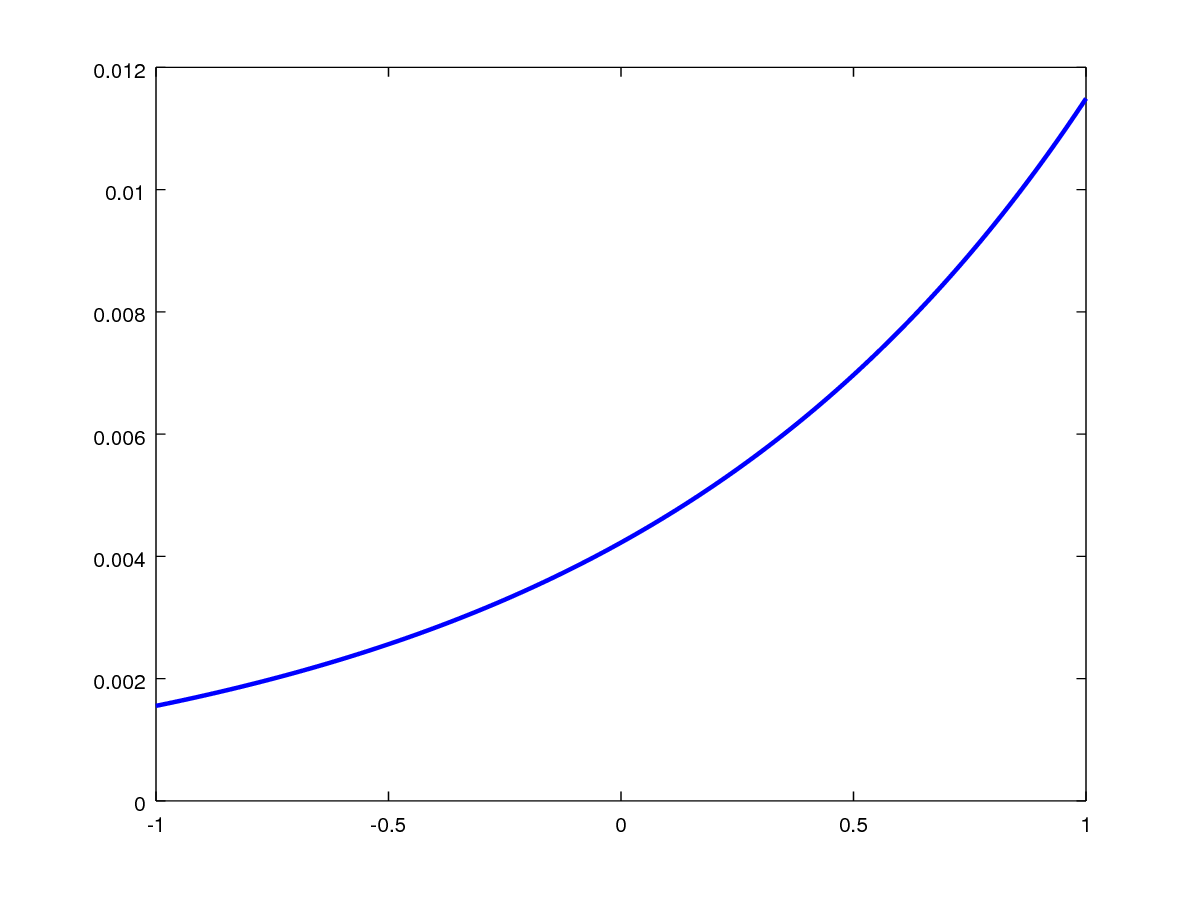
\includegraphics[width=1\linewidth]{figures/softmax.png}
			\caption{Softmax activation function}\label{fig:softmax}
		\end{subfigure}
		\caption[Activation functions]{}
		\label{fig:activations}
	\end{figure}
	
\end{description}

\begin{description}
	\item[Flatten layer] It \textit{flattens} the input. For instance, it converts the activation maps returned by the convolutional layers into a \textbf{vector of neurons} before being connected to a dense layer. It takes no arguments.
\end{description}

\begin{description}
	\item[Dropout layer] It's considered a \textbf{regularization layer}, because its main purpose is to avoid over-fitting. Dropout \cite{Srivastava-et-al-2014} is a technique that randomly \textbf{\textit{switches-off}} a fraction of hidden units during training, both forward and backward propagation. Another point of view of how dropout works can be seen in figure \ref{fig:dropout}.

	\begin{figure}
		\centering
		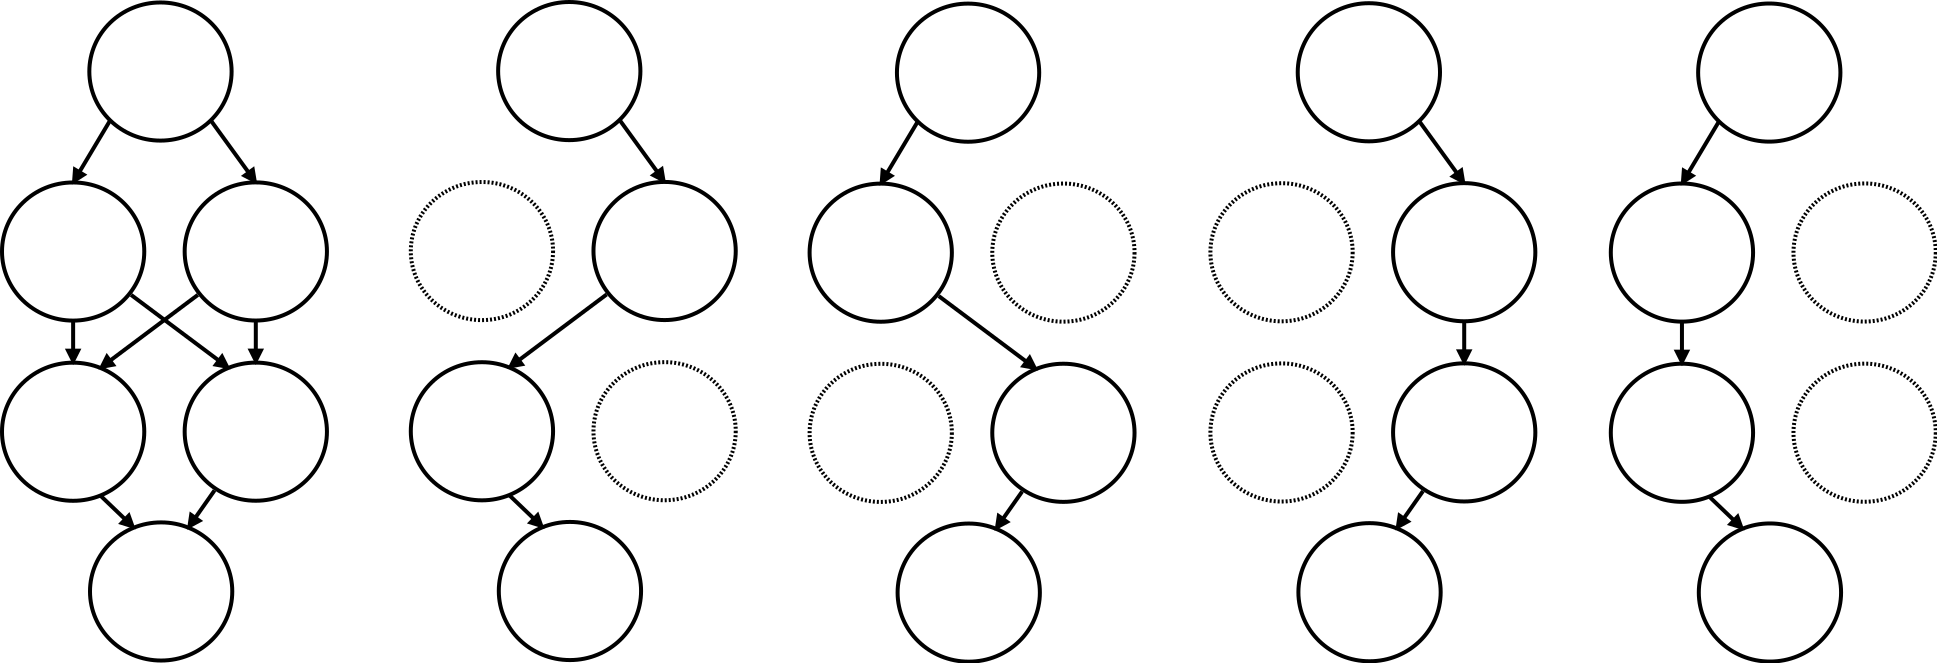
\includegraphics[width=1\linewidth, keepaspectratio]{figures/dropout.png}
		\caption[Subnetworks generated when using dropout]{Dropout can be understood as a technique that "trains an ensemble consisting of all subnetworks that can be structured by removing non-output units from an underlying base network" \cite{Goodfellow-et-al-2016}.}
		\label{fig:dropout}
	\end{figure}	

	 This layer, as other regularization layers (i.e. GaussianNoise layer), is only active during training. It's main argument is:
	\begin{itemize}
		\item \textbf{\textit{rate}}: fraction of units that must be dropped.
	\end{itemize}
	
\end{description}

\subsection{Callbacks} \label{subsec:callbacks}
As defined by Keras documentation \cite{chollet2015keras}, \textbf{callbacks} are a set of functions which are applied at given stages while the model is being trained. They can be used to take a look at the state of the model during training. The built-in callbacks that have been used for this project are:
\begin{itemize}
	\item \textbf{\textit{.History()}}: it is automatically applied to every Keras model and is returned by the \textit{.fit()} method. It evaluates the declared metrics with the validation set after each epoch and saves the results.
	
	\item \textbf{\textit{.EarlyStopping()}}: it monitors the value of a given metric and forces the model to stop training when that metric has stopped improving. It has a \textbf{\textit{patience}} argument which determines how many epochs in a row without improving must be tolerated before the model quits training. Setting up an appropriate \textbf{stopping criteria} may prevent the model from over-fitting.
	
	\item \textbf{\textit{.ModelCheckpoint()}}: it saves the model and its weights after each epoch. It can be configured to overwrite the model only if a certain metric has improved with respect to the previous best result, saving the best \textit{version} of it.
\end{itemize}

Additionally, Keras provides the \textit{Callback} base class that can be used to build \textbf{user-defined callbacks}.

\subsection{Image Preprocessing}
\textbf{Image preprocessing} is a key factor in every computer vision application. Specifically, in machine learning, besides adapting the image and extracting features before the training that can improve the model performance (i.e. edge extraction), it can be used to avoid \textbf{over-fitting} through data augmentation. \textbf{Data augmentation} \cite{DBLP:journals/corr/WongGSM16} consists in taking the samples that the dataset already contains and applying transformations to them, generating new samples that may be closer to real world and, in any case, enlarging the dataset with new data.

This functionality is included in Keras thanks to the \textbf{\textit{.ImageDataGenerator()} method}. It returns a batch generator which randomly applies the desired \textbf{transformations} to random samples of the dataset provided by the user. Built-in transformations like rotation, shifting and zooming, are passed as arguments to the aforementioned method. Additionally, it's possible to build a user-defined function and pass it as an argument as well. The dataset, and the batch size are defined through the \textbf{\textit{.flow()} method}. During training, the generator will loop until the number of samples per epoch and the number of epochs set by the user are satisfied.

\subsection{Utils}
Keras include a module for multiple supplementary tasks called \textbf{\textit{Utils}}. The most important functionality for the project provided by this module is the \textbf{\textit{.HDF5Matrix()} method}. It reads the \textbf{HDF5 datasets} \ref{sec:hdf}, which are going to be used as inputs to the neural networks.

\section{HDF5}\label{sec:hdf}
During the development of this project, \textbf{huge amounts of data} have been processed. That's why an efficient way of reading and saving this data has been an important point. Keras employs the \textbf{HDF5 file format} to save models and read datasets.

According to HDF5 (Hierarchical Data Format) documentation \cite{hdf5}, it is designed for high volumes of data with complex relationships. While relational databases employ tables to store data, HDF5 supports \textbf{n-dimensional datasets} and each element in the dataset may be as complex as needed.

In order to deal with HDF5 files, the \textbf{h5py} \footnote{\url{http://www.h5py.org/}} library for Python has been employed.

\section{Scikit-learn}\label{sec:sklearn}
\textbf{Scikit-learn} \cite{scikit-learn} is a \textbf{machine learning library} that includes a wide variety of algorithms for clustering, regression and classification. It can be used during the whole machine learning process: preprocessing, training, model selection and evaluation.

Scikit-learn functions have been used to evaluate the neural networks developed with Keras. Using a tool that is \textbf{independent from Keras} enables the comparison of the results achieved by different neural network libraries (e.g. Keras and Caffe). These are the \textbf{metrics} employed in this project (equations obtained from \cite{scikit-doc}):
\begin{itemize}
	\item \textbf{Precision}: ability of the classifier not to label as positive a sample that is negative.
	\begin{equation}\label{eq:precision}
	\textrm{precision}=\frac{true_{positives}}{true_{positives}+false_{positives}}
	\end{equation}
	
	\item \textbf{Recall}: ability of the classifier to find all the positive samples.
	\begin{equation}\label{eq:recall}
	\textrm{recall}=\frac{true_{positives}}{true_{positives}+false_{negatives}}
	\end{equation}
	
	\item \textbf{Confusion matrix}: a matrix where the element $i,j$ represents the number of samples that belongs to the group $i$ but has been classified as belonging to group $j$. True predictions can be found in the diagonal of the matrix, where $i=j$. An example of a confusion matrix constructed with Scikit-learn and displayed with Octave \ref{sec:octave} can be found in figure \ref{fig:conf_mat}.
\end{itemize}

Besides the metrics that have just been mentioned, \textbf{accuracy} and \textbf{log loss} have also been used and they're defined as in section \ref{subsec:models}.

\section{Octave} \label{sec:octave}
\textbf{GNU Octave} \cite{octave} is a scientific programming language compatible with \textbf{Matlab}. It provides powerful tools for \textbf{plotting}, which have been used to visualize the data collected with Scikit-learn about the performance of the models. An example of Octave usage can be seen in the figure \ref{fig:conf_mat}.
\begin{figure}
	\centering
	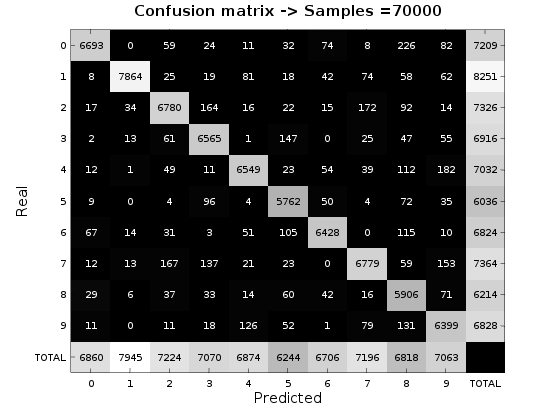
\includegraphics[width=12cm, keepaspectratio]{figures/conf_mat.png}
	\caption{Example of a confusion matrix visualization using Octave}
	\label{fig:conf_mat}
\end{figure}
\lhead[]{CHAPTER \thechapter. DIGIT CLASSIFIER}
\include{4-Digit_classifier}
\lhead[]{CHAPTER \thechapter. EVALUATION}
\chapter{Evaluation}\label{sec:new_models}
The \gls{cnn} analyzed in Section~\ref{sec:understanding} is going to be taken as a starting point to build \emph{new models}. These models will be trained with different datasets and regularization methods and, finally, new architectures will be implemented. In this chapter, the tools developed in Chapter~\ref{ch:benchmark} will be employed to evaluate the results achieved by each \gls{cnn}. These tests will serve as a way to study the effects of the learning process in these algorithms. Before talking about the \emph{performance} of the new models, the visualization of the convolutional layers filters and activation maps is going to be analyzed.

\section{Convolutional layers visualization}
The filters and activation maps discussed in this section belong to the convolutional layers of the \emph{\textit{0-1; Patience=2} model} that can be found in Section~\ref{subsec:early_stopping}. This model has been trained with the \textit{0-1} dataset (see Section~\ref{subsec:handmade}) and an early stopping rule with patience~2. Its architecture corresponds to the one defined in Section~\ref{sec:understanding}. In order to generate the activation maps, the model will be fed with a sample extracted from the \textit{0-1} dataset. It can be seen in Figure~\ref{fig:sample}.
\begin{figure}
	\centering
	\includegraphics[width=0.3\linewidth, keepaspectratio]{figures/0-1_sample.png}
	\caption{Sample employed to generate the activation maps.}
	\label{fig:sample}
\end{figure}

\subsection{Filters}
When loading the weights of the \emph{first convolutional layer}, a Numpy array of shape~(1,~3,~3,~32) is obtained. This means that the weights are arranged in~32~filters of size~3x3. In this case, the input is a grayscale image, so the filters only have one channel (i.e. depth=1). Besides that, when examining their values, \emph{negative and positive coefficients} are found.

In Figure~\ref{fig:filters}, these filters are plotted. Some of the filters look too noisy to tell which kind of feature they are looking for. However, a few of them can be interpreted at first sight as follows:
\begin{itemize}
	\item \textbf{Horizontal edge-emphasizing filter}: filters~7,~9~and~23.
	\item \textbf{Vertical edge-emphasizing filter}: filters~8,~15~and~31.	
\end{itemize}

\begin{figure}
	\centering
	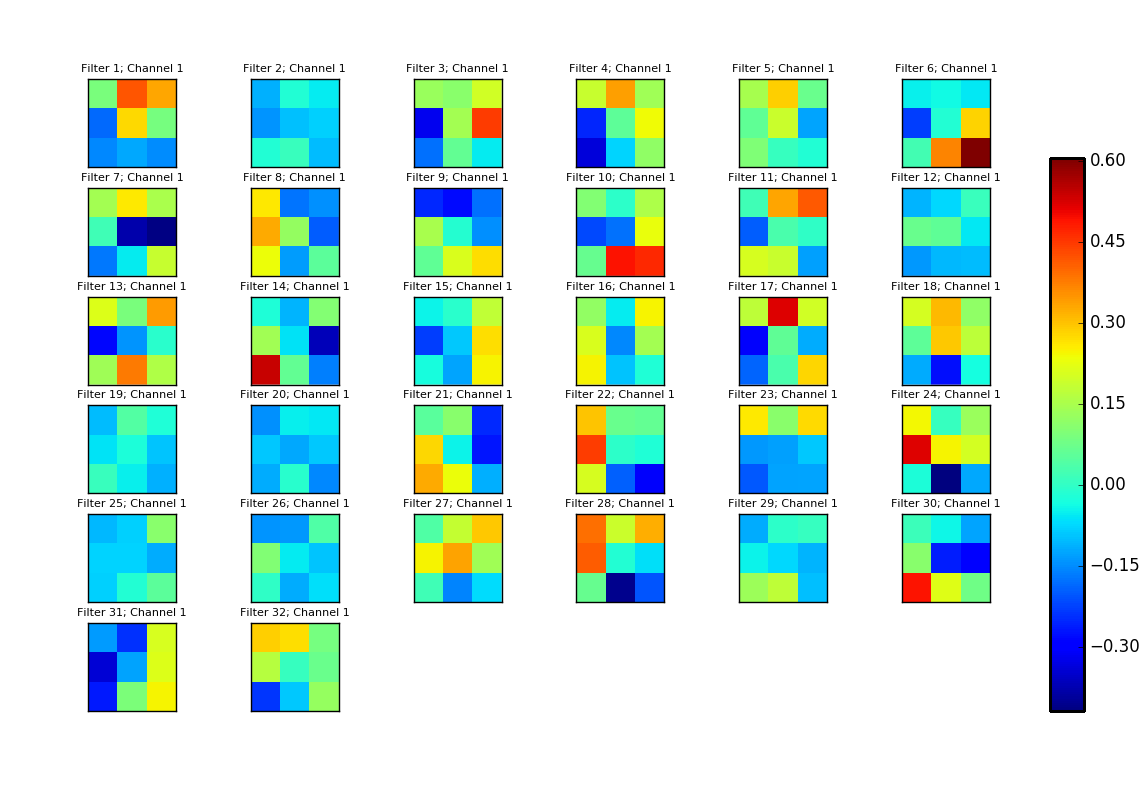
\includegraphics[width=0.92\linewidth, keepaspectratio]{figures/weights_conv2d_1.png}
	\caption{Filters of the first convolutional layer.}
	\label{fig:filters}
\end{figure}

The filters in the \emph{second convolutional layer} have been displayed as well. The weights in this layer are stored in a Numpy array of shape~(32,~3,~3,~32), which means that there are~32~filters with size~3x3~as well. However, this time their depth is~32, since there is one channel per activation map generated by the previous layer. As we get deeper in the \gls{cnn} and the dimensionality grows, the filters look noisier and become harder to interpret, as it is shown in Figure~\ref{fig:filters2}.
\begin{figure}
	\centering
	\includegraphics[width=1\linewidth, keepaspectratio]{figures/weights_conv2d_2_mod.png}
	\caption{Filters of the second convolutional layer.}
	\label{fig:filters2}
\end{figure}

\subsection{Activation maps}
Figure~\ref{fig:activation_maps} shows the activation maps that the \emph{first convolutional layer} of the model outputs. There are \emph{horizontal and vertical edge images} that confirm the interpretation of the filters given in the previous section. Besides that, some activation maps (2,~12,~19,~25~and~26) look \textit{dead}. If we look back into Figure~\ref{fig:filters}, these activation maps correspond to filters with \emph{almost flat coefficients}. This may be a signal of a high learning rate~\cite{cs231n}. In this case, the learning rate is not explicitly declared, because the ADADELTA optimizer uses an adaptive one.
\begin{figure}
	\centering
	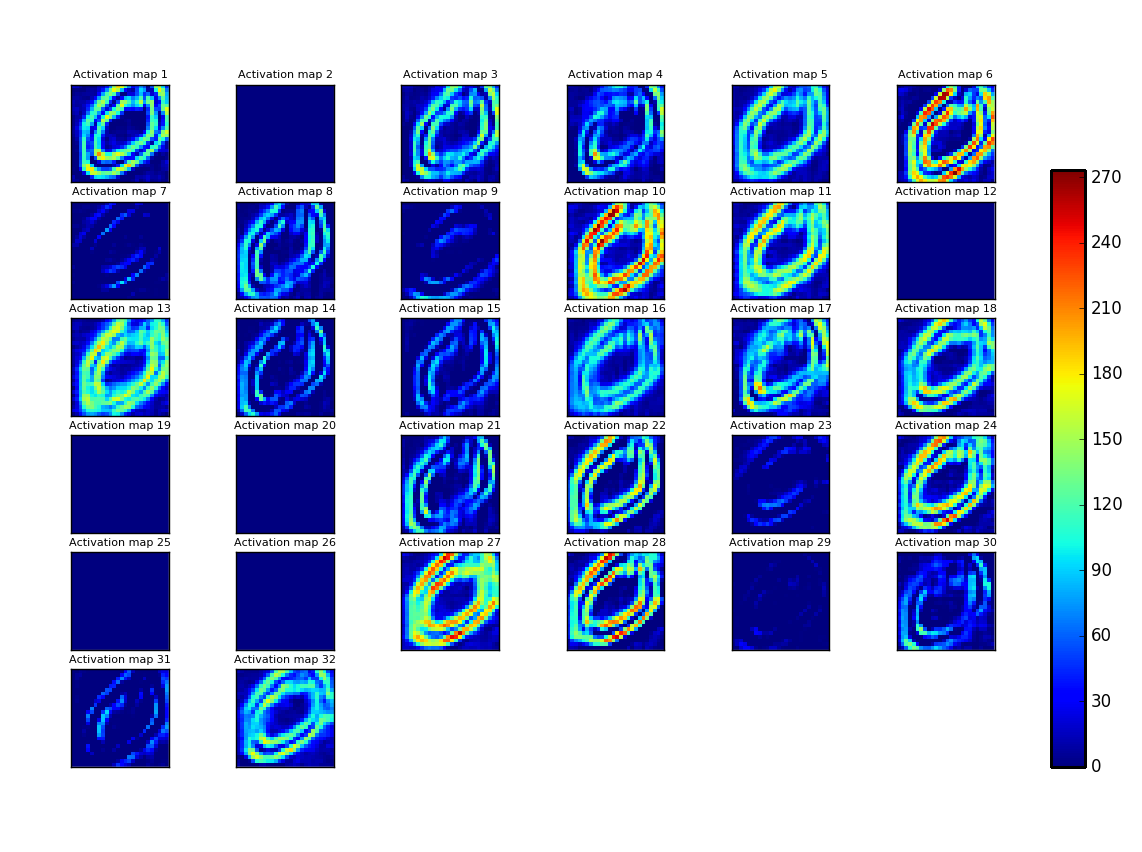
\includegraphics[width=0.9\linewidth, keepaspectratio]{figures/activation_maps_conv2d_1.png}
	\caption{Activation maps of the first convolutional layer.}
	\label{fig:activation_maps}
\end{figure}

The activation maps of the \emph{second layer} are shown in Figure~\ref{fig:activation_maps2}. The images obtained look \emph{more specialized} than the ones in the previous layer. It's easier to tell to what kind of feature (e.g. edges and corners) each activation map is responding to.
\begin{figure}
	\centering
	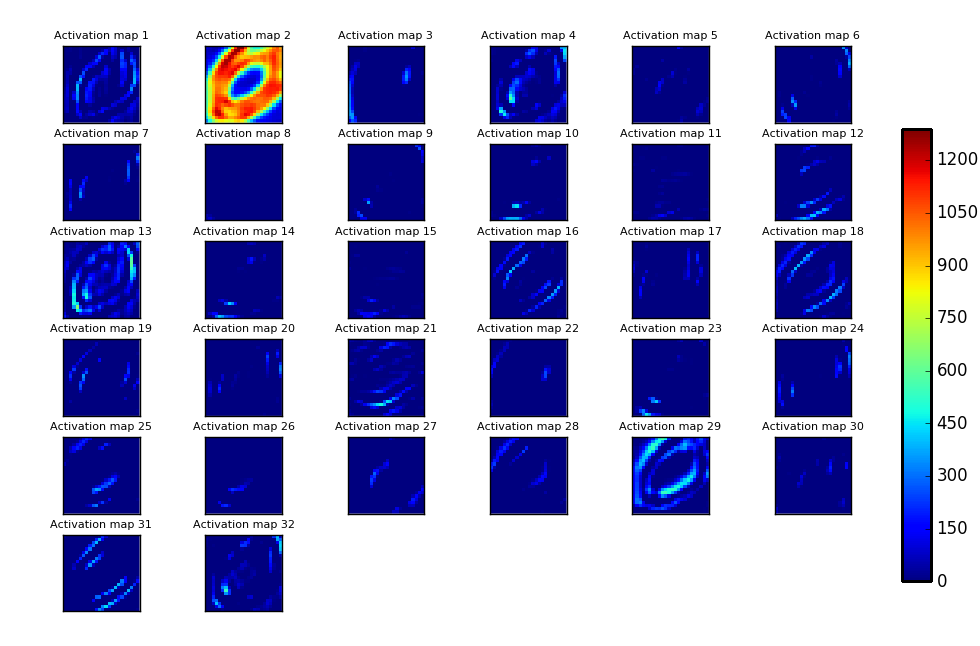
\includegraphics[width=0.9\linewidth, keepaspectratio]{figures/activation_maps_conv2d_2.png}
	\caption{Activation maps of the second convolutional layer.}
	\label{fig:activation_maps2}
\end{figure}

It's important to note that the values of the activation maps are \emph{always positive}, even if the filters have negative coefficients. This is because the \gls{relu} activation function (see Equation~\ref{eq:relu}) turn all the negative values to zero.

\section{Augmented datasets}\label{sec:new_datasets}
The original model has been trained with each of the \emph{handmade datasets} described in Section~\ref{sec:datasets}. The number of epochs has been set to~12~and the evaluation has been carried out with the~\emph{1-6~test dataset}. The results that can be seen in Table~\ref{tbl:datasets} lead to the following conclusions:
\begin{itemize}
	\item As it might be expected, the results when training with the \emph{Sobel dataset} are much worse than the ones obtained with the other datasets, because we're testing with noisy images a \gls{cnn} trained with noiseless samples.
	\item The \emph{\textit{0-6} and \textit{1-6} models} are the ones that achieve better results, as they have been trained with much more samples than \textit{0-1} and \textit{1-1}.
	\item When \emph{comparing \textit{0-1} with \textit{1-1} and \textit{0-6} with \textit{1-6}}, it can be seen that the performance is almost the same, which means that the gradient image without noise and transformations is not adding much information to the model.
\end{itemize}
In Figure~\ref{fig:val_datasets}, the validation results obtained after every epoch when training the model with each dataset can be seen.
\begin{figure}
	\centering
	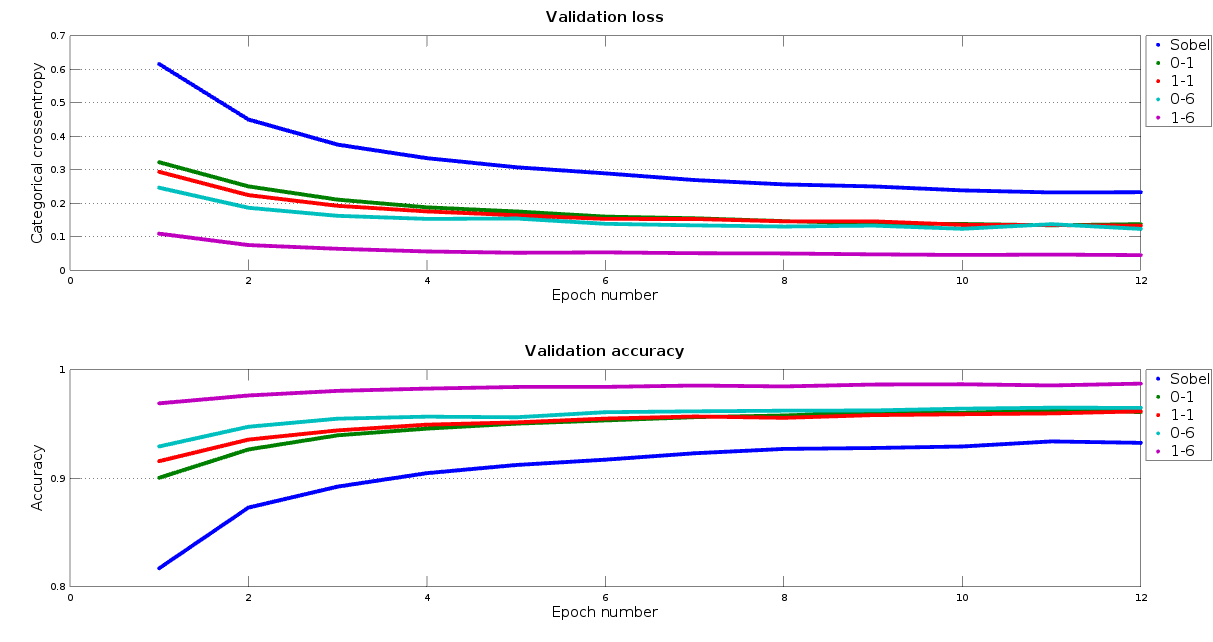
\includegraphics[width=1\linewidth, keepaspectratio]{figures/val_datasets.png}
	\caption{Validation results when training the model with different datasets.}
	\label{fig:val_datasets}
\end{figure}

Taking all of this into account, it has been decided to keep working with the \emph{\textit{0-1} model}, which achieves a performance that is comparable with the other models with the advantage of a much lower computational cost.

\begin{table}
	\centering
	\begin{tabular}{l*{4}{c}r}
		\textbf{Model} & \textbf{Loss} & \textbf{Accuracy} & \textbf{Epochs} \\
		\hline
		Sobel & 1.233 & 0.699 & 12 \\
		0-1 & 0.201 & 0.939 & 12 \\
		1-1 & 0.189 & 0.943 & 12 \\
		0-6 & 0.109 & 0.968 & 12 \\
		1-6 & 0.111 & 0.967 & 12 \\
	\end{tabular}
	\caption{Results of training with different datasets.}
	\label{tbl:datasets}
\end{table}

\section{Regularization methods}
``\emph{Regularization} is any modification we make to a learning algorithm that is intended to reduce its \emph{generalization error} but not it's training error"~\cite{Goodfellow-et-al-2016}. Reducing the generalization error is important because, even if a model achieves a great accuracy or loss with the training dataset, if it doesn't generalize well enough, the results during validation and test time won't be optimal. This is specially significant in our case, since the predictions of the digit classifier will be based on images that differ a lot from the training dataset. In this section, the effects of applying to the \emph{\textit{0-1} model} two regularization techniques (early stopping and dropout) are going to be evaluated. 

\subsection{Early stopping}\label{subsec:early_stopping}
The models in the previous section have been trained for~12~epochs. However, if we look at the \emph{validation results} in Figure~\ref{fig:val_datasets}, it can be assumed that the models were \emph{not overfitting} yet, because the results didn't stop improving. This means that they were not being trained as much as possible. Setting an \emph{early stopping} rule (see Section~\ref{subsec:callbacks}) allows training the \gls{cnn} right until it starts to overfit, making the most of it. The criteria that has been used depends on the loss during validation. The model is trained until the \emph{log loss} (see Section~\ref{eq:categorical_crossentropy}) has not improved after two validations in a row, which means a \textit{patience} of 2. Besides that, in order to keep the best \textit{version} of the model, the log loss is checked after each epoch and, if the value is lower than the previous best log loss achieved, the weights of the model are saved, overwritting the weights of the previous best \textit{version}. The difference between training the model with and without early stopping can be seen in Table~\ref{tbl:earlystopping}.
\begin{table}
	\centering
	\begin{tabular}{l*{4}{c}r}
		\textbf{Model} & \textbf{Loss} & \textbf{Accuracy} & \textbf{Epochs} \\
		\hline
		0-1 & 0.201 & 0.939 & 12 \\
		0-1; Patience=2 & 0.155 & 0.954 & 30 \\
	\end{tabular}
	\caption{Results of training with and without early stopping.}
	\label{tbl:earlystopping}
\end{table}

Early stopping means an improvement of 1.6\% in accuracy and 4.6\% in log-loss. The model has been trained for~30~epochs and it reached its best \textit{version} at the 27$^{th}$ epoch. Setting a longer \textit{patience} has been considered, but it has been decided to apply it only to the best model obtained in Section~\ref{subsec:arch} to reduce the computational cost.

\subsection{Dropout}
The models that have already been evaluated insert \emph{dropout} (see Section~\ref{subsec:layers}) before every dense layer of the \gls{cnn} (0.25\% and 0.5\%, respectively). Dropout is usually applied just to fully-connected or \emph{dense layers}, because convolutional layers are less likely to overfit due to their architecture. In order to determine how dropout affects the performance of the \glspl{cnn}, the \emph{\textit{0-1; Patience=2} model}, defined in the previous section, has been trained with and without the mentioned dropout. The results can be seen in Table~\ref{tbl:dropout}. 
\begin{table}
	\centering
	\begin{tabular}{l*{4}{c}r}
		\textbf{Model} & \textbf{Loss} & \textbf{Accuracy} & \textbf{Epochs} \\
		\hline
		No dropout & 0.189 & 0.945 & 9 \\
		Dropout & 0.155 & 0.954 & 30 \\
	\end{tabular}
	\caption{Results of training with and without dropout.}
	\label{tbl:dropout}
\end{table}

Without dropout, the model has stopped training after~9~epochs. It has \emph{learned faster}, but it has started \emph{overfitting} earlier, resulting in worst results that the ones achieved by the model trained with dropout. This can be clearly seen in Figure~\ref{fig:comp_dropout}
\begin{figure}
	\centering
	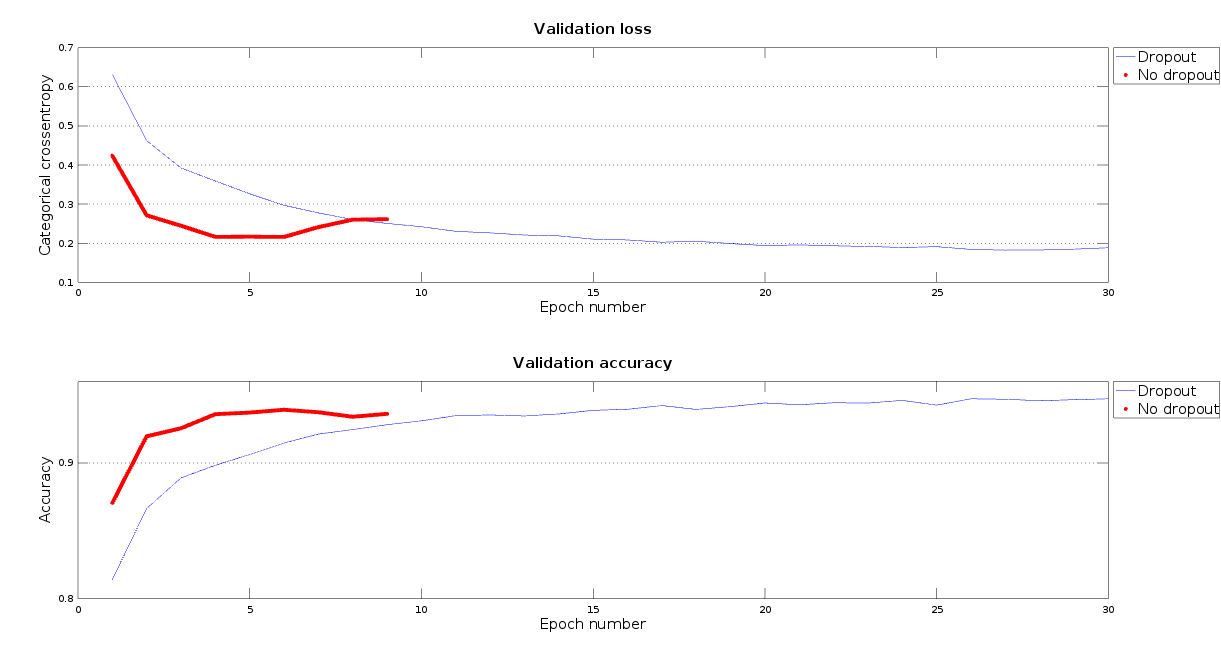
\includegraphics[width=1\linewidth, keepaspectratio]{figures/comp_dropout.png}
	\caption{Validation results with and without dropout.}
	\label{fig:comp_dropout}
\end{figure}

Additionally, in Figure~\ref{fig:lc_dropout}, the learning curves of both models can be seen. It's worth looking into these plots to realize that validation results are better than training results when the model is trained with dropout. This may seem illogical, as the \gls{cnn} should always perform better with samples that it has already seen. However, it's important to remember that dropout only applies during training and, as it will \textit{switch-off} a lot of weights in the \gls{cnn}, much of its prediction power will be lost. During validation, there are no \textit{switched-off} weights, which allows the \gls{cnn} to make better predictions. Besides that, in the figure can be seen that the training results are better when the model is trained without dropout, while the validation results are better with dropout. This means that the model with dropout is \emph{generalizing} better than the one without dropout. 
\begin{figure}
	\begin{subfigure}{1\textwidth}
		\centering
		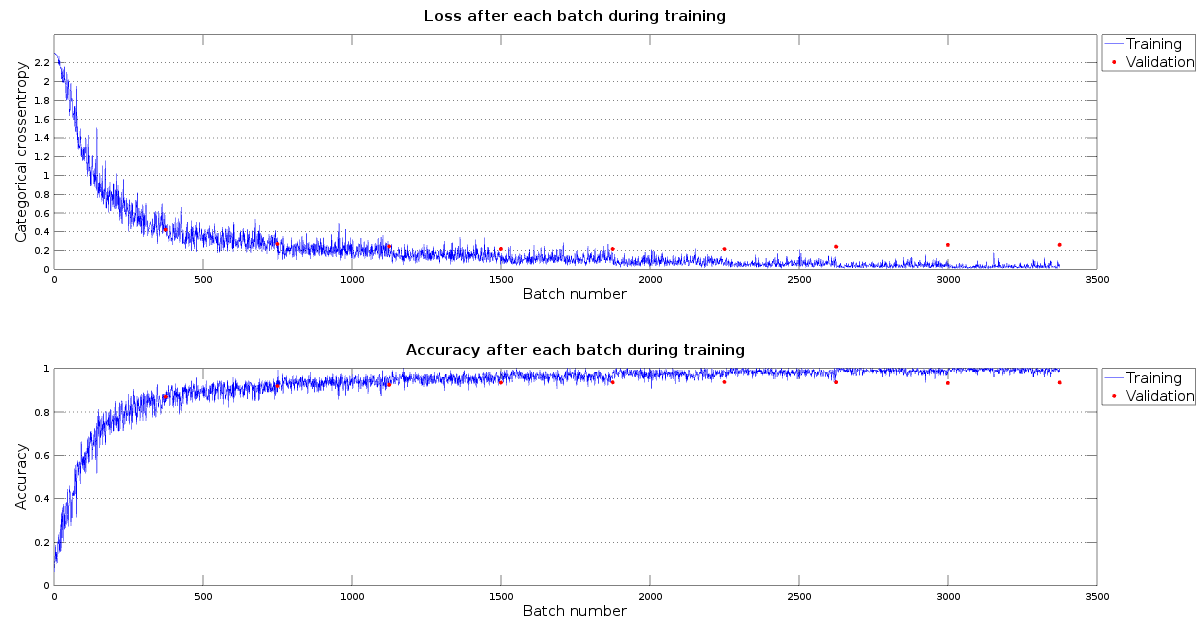
\includegraphics[width=1\linewidth]{figures/lc_nodropout.png}
		\caption{}
	\end{subfigure}
	\begin{subfigure}{1\textwidth}
		\centering
		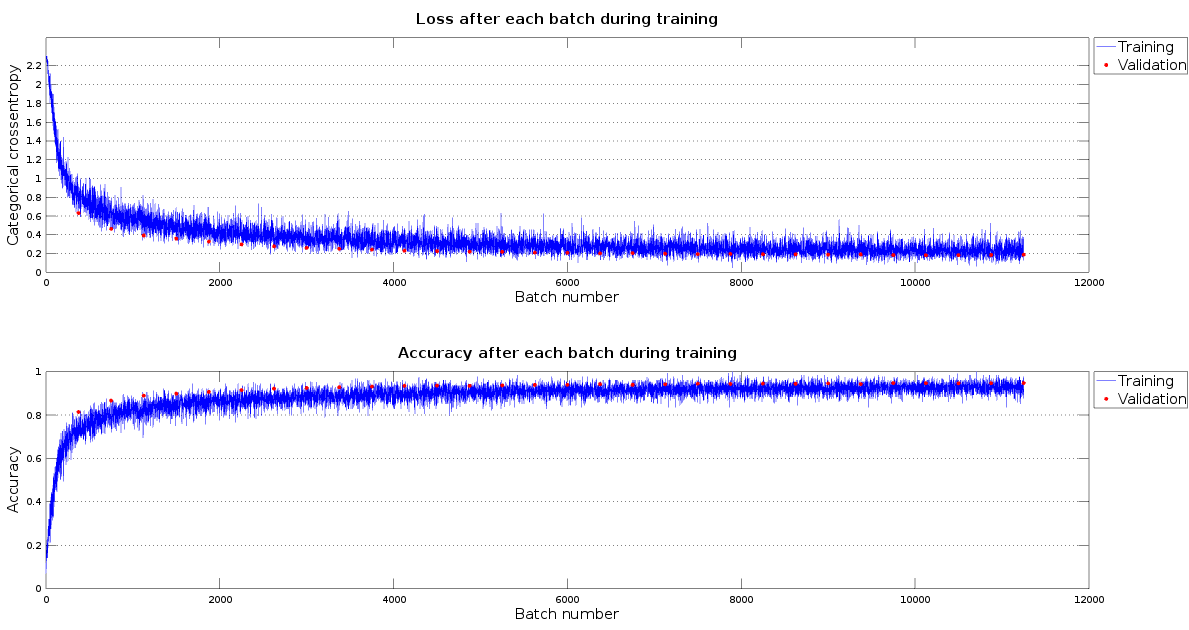
\includegraphics[width=1\linewidth]{figures/lc_dropout.png}
		\caption{}
	\end{subfigure}
	\caption{Learning curves: (a) without dropout; (b) with dropout.}
	\label{fig:lc_dropout}
\end{figure}

\section{New architectures}\label{subsec:arch}
In order to check the influence of \emph{different architectures} in the performance of the \gls{cnn}, new models with a different number of convolutional layers have been trained and tested. The stopping rule used in these trainings is the one defined in Section~\ref{subsec:early_stopping} and dropout is also applied. The decision of adding \emph{pooling layers} to the models (see Section~\ref{subsec:layers}) has been taken to reduce computational cost. In the first attempt at training a model with~6~convolutional layers, the model with~2~convolutional layers and one \emph{MaxPooling layer} was triplicated. However, the first MaxPooling layer of the model was removed because the model ended up working with an empty image:~0x0~size.
\begin{table}
	\centering
	\begin{tabular}{l*{4}{c}r}
		\textbf{Model} & \textbf{Loss} & \textbf{Accuracy} & \textbf{Epochs} \\
		\hline
		1Conv+MaxPooling & 0.191 & 0.945 & 47 \\
		2Conv+MaxPooling & 0.155 & 0.954 & 30 \\
		3Conv+MaxPooling & 0.129 & 0.945 & 28 \\
		2Conv+MaxPooling+2Conv+MaxPooling & 0.092 & 0.970 & 27 \\
		4Conv+MaxPooling+2Conv+MaxPooling & 0.092 & 0.971 & 24 \\
	\end{tabular}
	\caption{Results of training models with different architectures.}
	\label{tbl:arch}
\end{table}

As it is shown in Table~\ref{tbl:arch}, the best results have been obtained with the models that contain~4~and~6~convolutional layers. Besides that, taking a look into the validation curves (see Figure~\ref{fig:comp_arch}), it can be assumed that when the number of layers is increased, the neural network tends to lead to better results with less epochs.

\begin{figure}
	\centering
	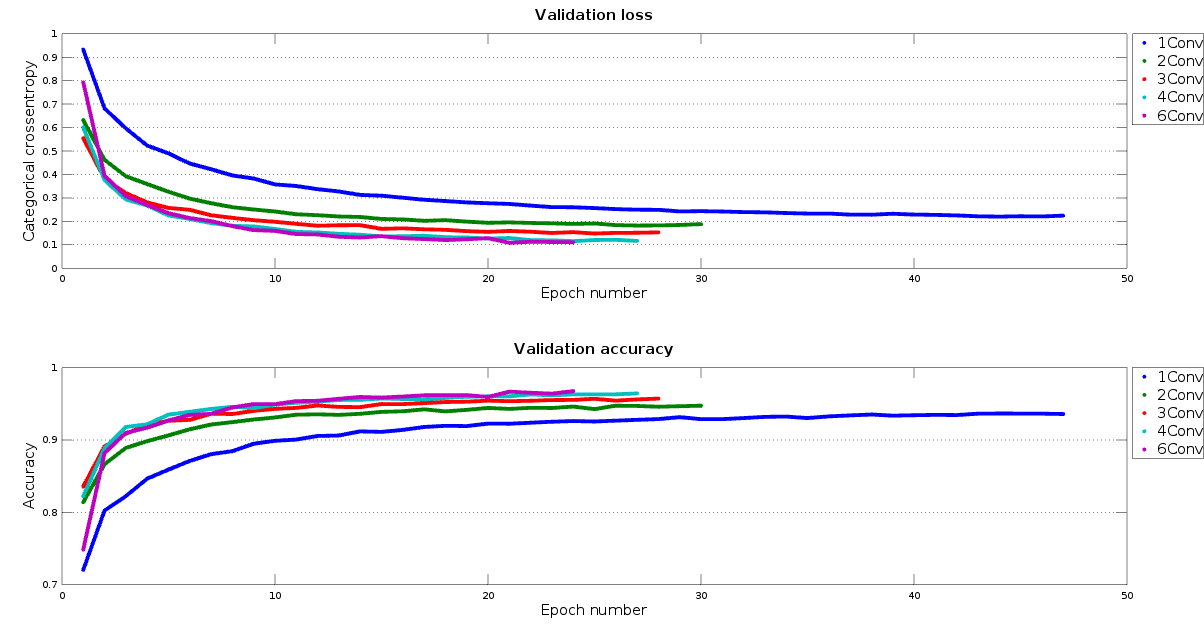
\includegraphics[width=1\linewidth, keepaspectratio]{figures/full_comparison.png}
	\caption{Validation results with different architectures.}
	\label{fig:comp_arch}
\end{figure}

The model with~6~layers has a slightly better accuracy, but a slightly worse loss, than the one with~4~layers. Considering that computational cost is higher when training the \textit{6Conv} model, the \emph{\textit{4Conv} model} seems to be the best bet. In order to make the most of it, it has been trained again but increasing the \emph{\textit{patience}} of the early stopping rule from~2~to~5. The results obtained with this new stopping rule can be seen in Table~\ref{tbl:arch_patience5}. These results imply that being more \textit{patient} during training can lead to a better performance, although in this case the improvement is not very significant.
\begin{table}
	\centering
	\begin{tabular}{l*{4}{c}r}
		\textbf{Model} & \textbf{Loss} & \textbf{Accuracy} & \textbf{Epochs} \\
		\hline
		4Conv; Patience=2 & 0.092 & 0.970 & 27 \\
		4Conv; Patience=5 & 0.082 & 0.973 & 37 \\
	\end{tabular}
	\caption{\textit{4Conv} model trained with different stopping rules.}
	\label{tbl:arch_patience5}
\end{table}

A visualization of the performance achieved by the best model built in this project (i.e. \emph{4Conv; Patience=5 model}) is shown in Figure~\ref{fig:best}. The Octave function discussed in Section~\ref{subsec:octave-func} has been employed to generate the plots displayed in this figure.

\begin{figure}
	\centering
	\begin{subfigure}{1\textwidth}
		\centering
		\includegraphics[width=1\linewidth]{figures/lc_42.png}
		\caption{}
	\end{subfigure}
	\begin{subfigure}{0.5\textwidth}
		\centering
		\includegraphics[width=0.9\linewidth]{figures/pr_42.png}
		\caption{}
	\end{subfigure}%
	\begin{subfigure}{0.5\textwidth}
		\centering
		\includegraphics[width=0.9\linewidth]{figures/cm_42.png}
		\caption{}
	\end{subfigure}
	\caption{Performance of \textit{4Conv; Patience=5} model: (a) learning curves; (b) precision and recall; (c) confusion matrix.}
	\label{fig:best}
\end{figure}
\lhead[]{CHAPTER \thechapter. CONCLUSION}
\include{6-Conclusion}

%%%%%%%%%%%%%%% Bibliography %%%%%%%%%%%%%%%
\printbibliography

\end{document}